\documentclass[hidelinks,12pt]{report}
\usepackage[a4paper,width=150mm,top=25mm,bottom=30mm]{geometry}
\usepackage[utf8]{inputenc}

\usepackage{graphicx}
\graphicspath{{images/}{../images/}}

\usepackage[table]{xcolor}
\usepackage{multirow,tabularx}
\newcolumntype{Y}{>{\centering\arraybackslash}X}

\usepackage{sectsty}
\allsectionsfont{\sffamily}

\usepackage[titletoc]{appendix}

\usepackage{natbib}
\setcitestyle{aysep={}}
% line break in bibliography urls
\usepackage{xurl}

\usepackage{caption}
\usepackage{tocbibind}

% indent paragraphs
\usepackage{changepage}

\usepackage{mathtools}
\usepackage{amsmath}
\usepackage{amssymb}
\usepackage{amsthm}
\usepackage{color}
\usepackage{float}
\usepackage{bm}
\usepackage{multirow, makecell}
\usepackage{enumitem}
\usepackage{bold-extra}
\usepackage[mathscr]{euscript}

% matrix with labeled rows and columns
\usepackage{kbordermatrix}

\usepackage[linesnumbered,ruled,vlined]{algorithm2e}
\SetKw{Continue}{continue}
\SetKw{Input}{Input:}
\SetKw{Output}{Output:}


\DeclareMathOperator{\lca}{lca}
\DeclareMathOperator*{\argmax}{arg\,max}
\DeclareMathOperator*{\argmin}{arg\,min}
\newcommand{\TODO}[1]{\begingroup\color{red}#1\endgroup}
\newcommand{\OLD}[1]{\begingroup\tiny   \color{green}#1\endgroup}
\newtheorem{theorem}{Theorem}
\newtheorem{lemma}[theorem]{Lemma}
\newtheorem{corollary}[theorem]{Corollary}
\newtheorem{definition}[theorem]{Definition}
\newtheorem{fact}[theorem]{Observation}
\def\arrowedvec{\mathaccent"017E}
\newcommand{\G}{\arrowedvec{G}}
\newcommand{\unrooted}[1]{\overline{#1}}  
\newcommand{\ROOT}{\circledcirc}
\newcommand{\LEAF}{\odot}
\usepackage{wasysym}
\newcommand{\SPEC}{\newmoon}
\newcommand{\HGT}{\triangle}
\newcommand{\DUPL}{\square}
\newcommand{\child}{\mathsf{child}}
\newcommand{\degree}{\mathsf{deg}}
\newcommand{\parent}{\mathsf{par}}
\newcommand{\bmr}{\mathrel{\bm{\rightarrow}}}
\newcommand{\C}[1]{\mathscr{C}_{#1}}
\newcommand{\AX}[1]{\textnormal{#1}}

% symbol for disjoint union
\makeatletter
\def\moverlay{\mathpalette\mov@rlay}
\def\mov@rlay#1#2{\leavevmode\vtop{%
		\baselineskip\z@skip \lineskiplimit-\maxdimen
		\ialign{\hfil$\m@th#1##$\hfil\cr#2\crcr}}}
\newcommand{\charfusion}[3][\mathord]{
	#1{\ifx#1\mathop\vphantom{#2}\fi
		\mathpalette\mov@rlay{#2\cr#3}
	}
	\ifx#1\mathop\expandafter\displaylimits\fi}
\makeatother
\newcommand{\cupdot}{\charfusion[\mathbin]{\cup}{\cdot}}

% Mark overfull boxes
\overfullrule=1mm

% Hyphenation and line breaks
\hyphenation{du-pli-ca-ti-on}

% contents links etc.
\usepackage{hyperref}
\hypersetup{
	colorlinks=True,
	linkcolor=blue,
	filecolor=magenta,      
	urlcolor=cyan,
	citecolor=black,
}

%\usepackage{setspace}

\begin{document}

\begin{titlepage}
	\begin{center}
		\includegraphics[width=0.4\textwidth]{logo.pdf}
	\end{center}
	\begin{center}
		\vspace*{1cm}
		
		\Huge
		\textsf{\textbf{AsymmeTree}}
		\vspace{1.5cm}
		
		\LARGE
		User Manual\\
		\vspace{1.0cm}
		\large
		David Schaller
		
		\vspace{1.0cm}
		\TODO{This manual is work in progress!}
		
	\end{center}
\end{titlepage}

\newpage

\tableofcontents

\chapter{Introduction}

AsymmeTree is Python library for the simulation and analysis of phylogenetic scenarios.
It includes a simulator for species and gene tree scenarios with asymmetric evolution rates, tools for the inference and analysis of best matches (resp. best hits) and orthology, as well as an algorithm to compute supertrees.

\chapter{Manual}

\section{Installation}

\subsection{Easy Installation with Pip}


The \texttt{asymmetree} package is available on PyPI:

pip install asymmetree

For details about how to install Python packages see
\href{https://packaging.python.org/tutorials/installing-packages/}{here}.

\subsection{Dependencies}

AssymmeTree has several dependencies (which are installed automatically when using \texttt{pip}):

\begin{itemize}
	\item \href{https://networkx.github.io}{NetworkX}
	\item \href{http://www.scipy.org/install.html}{SciPy and NumPy}
	\item \href{https://matplotlib.org/}{Matplotlib}
\end{itemize}

Furthermore, to use functions involving sequence simulation and alignment, the following packages must be installed (i.e., they are not installed automatically!):

\begin{itemize}
	\item \href{http://biopython.org/wiki/Download}{Biopython}
	\item \href{https://github.com/sjspielman/pyvolve}{Pyvolve}
\end{itemize}

To use the tree reconstruction method for best match inference and the C++ implementation of the quartet method, resp., the following software must be installed
(I recommend that you compile these tools on your machine, place the binaries into a persistent location and add this location to your PATH environment variable):

\begin{itemize}
	\item \href{https://birc.au.dk/software/rapidnj/}{RapidNJ}
	\item \href{https://github.com/david-schaller/qinfer}{qinfer}
\end{itemize}


\section{Overview}

\subsection{Tree Data Structures}

The two classes \texttt{Tree} (in \texttt{asymmetree.tools.Tree}) and \texttt{PhyloTree} (in \texttt{asymmetree.tools.PhyloTree}, inherits from \texttt{Tree}) implement tree data structures which are essential for most of the modules in the package.
The latter contains converters and parsers for the Newick format and a NetworkX graph format.

\subsection{Simulator for Species and Gene Trees}

The following steps are implemented in the Python package \texttt{asymmetree.simulator}:
\begin{itemize}
	\item species tree simulation ('innovation model')
	\item gene tree simulation (Gillespie algorithm)
	\item gene tree imbalancing (asymmetric evolution rates of paralogous genes)
	\item computation of a (noisy) distance matrix from the gene tree
\end{itemize}
 

\subsection{Best Match Inference}

Inference of the best match relation either directly from the gene tree or from a distance matrix (several methods).
\begin{itemize}
	\item \texttt{asymmetree.best\_matches}
\end{itemize}

References:
\begin{itemize}
	\item \citet{geiss2019a}
	\item \citet{geiss2020b}
	\item \citet{geiss2020c}
	\item \citet{stadler2020}
\end{itemize}

\subsection{Supertree Computation}

Implementation of the BuildST algorithm described by \citet{deng2016} to compute a supertree from a given list of tree based on the leaf labels. The algorithm uses the dynamic graph data structure described by \citet{henzinger1995} and \citet{holm2001}.
\begin{itemize}
	\item \texttt{asymmetree.tools.BuildST}
	\item \texttt{asymmetree.tools.hdtgraph.DynamicGraph}
\end{itemize}


\subsection{Cograph Editing and ParaPhylo}

The subpackages \texttt{asymmetree.cograph} and \texttt{asymmetree.proteinortho} contain heuristics for cograph editing and a method to compute rooted species tree from orthology/paralogy relations.
The latter is a reimplementation of \href{http://pacosy.informatik.uni-leipzig.de/208-0-ParaPhylo.html}{ParaPhylo} \citep{hellmuth2015} which uses heuristics for the NP-hard steps instead of exact ILP solutions.




\chapter{Detailed Description}

\section{Mathematical Preliminaries}
\label{sec:prelim}

\subsection{Graph and Tree Notation}
In this section, a very short introduction into the field of graph theory is given with a focus on the concepts that will be relevant in the subsequent sections.
For standard textbooks see e.g.\ \cite{diestel2017} and \citet{semple2003} from which definitions in the following were taken. The notation concerning trees follows the one used by \citet{geiss2019a}.

\begin{definition}[(Di-)Graph]
	A \emph{graph} is a pair $G=(V,E)$ of sets such that $E \subseteq [V]^2$, i.e., the elements of $E$ are 2-element subsets of $V$. The elements in $V$ are called vertices or nodes and the elements in $E$ are called edges. Here, an (undirected) edge $e$ between vertices $x$ and $y$ is written as $xy$.
	
	A \emph{directed graph} (or \emph{digraph}) is s graph that assigns to every edge an initial and terminal vertex. In this case, an edge $e$ is written as $(x,y)$ if $x$ is the initial, and $y$ is the terminal vertex of edge $e$.
\end{definition}

As usual, it is often written $V(G)\coloneqq V$ and $E(G)\coloneqq E$ for the sets of vertices and edges of a graph $G=(V,E)$ in order to express affiliation. Two vertices $x$ and $y$ are \emph{adjacent} if $xy\in E(G)$ [or $(x,y)\in E(G)$, respectively]. The \emph{degree} of a vertex $x$ is the number of adjacent vertices and denoted by $\degree(x)$.

The notation $G[x_1,...,x_k]$ refers to an induced subgraph $G'$ of a graph $G$ on the set $V(G')=\{x_1,...,x_k\}\subseteq V(G)$. Induced subgraphs are defined in the usual sense, i.e., $xy\in E(G')$ [or $(x,y)\in E(G')$ if $G$ is directed] if and only if $xy\in E(G)$ [$(x,y)\in E(G)$] and $x,y\in V(G')$.

An undirected graph $G=(V,E)$ is called \textit{connected} if any two vertices $x,y \in V(G)$ are linked by a path in $G$, i.e., there is a path $x=x_1-x_2-...-x_k=y$ such that $x_ix_{i+1} \in E(G)$ for all $1 \le i < k$.
A maximal connected subgraph of $G$ is called a \textit{connected component} of $G$. In case of a directed graph $\G$, a subgraph $\G^*$ of $\G$ is called a \textit{strongly connected component} if for any two vertices $x$ and $y$ there is directed path $x=x_1 \rightarrow x_2\rightarrow ...\rightarrow x_k=y$ such that $(x_i,x_{i+1}) \in E(\G)$ for all $1 \le i < k$ and vice versa. Furthermore, $\G^*$ must be maximal in that sense.

Given a non-empty set of colors $\mathcal{C}$, a \emph{proper vertex coloring} of a (di-)graph $G$ is a map $\sigma \colon V(T) \to \mathcal{C}$ such that $xy \in E(G) \implies \sigma(x) \ne \sigma(y)$. In other words, two adjacent vertices must not have the same color.

\begin{definition}[Rooted tree]
	A graph $T=(V,E)$ is a \emph{tree} if it is connected and acyclic. A \emph{rooted tree} is a tree $T$ with a special node $\rho$ called the \emph{root}. As a consequence of this, a partial order $\preceq_T$ on the vertex set $V(T)$ can be defined where $v \preceq_T u$ if $u$ lies on the (unique) path from $\rho$ to $v$.
\end{definition}

A vertex $u$ is called an \textit{ancestor} of $v$ in $T$ if $v \preceq_T u$, whereas $v$ is a descendant of $u$ in this case. If furthermore $uv \in T$, then $u$ is the parent of $v$, and $v$ is a child of $u$. The set of all children of a vertex $u$ is denoted by $\child(u)$. Likewise, $\parent(v)$ refers to the unique parent of a vertex $v$. It is set $\parent(v)=\emptyset$ if $v$ has no parent, i.e., $v$ is the root.

The set of all outer vertices $v \in V(T)$ (i.e., for which $\deg(v)=1$) is called the \textit{leaf set} of $T$ and denoted by $L(T)$. Hence, the leafs $L(T)$ are the minima and $\rho$ is the unique maximum w.r.t.\ $\preceq_T$.
The set of inner vertices $V(T)\setminus L(T)$ is denoted by $V^0(T)$, and a subtree of $T$ which is rooted at a vertex $u \in V^0(T)$ and contains all nodes and edges below $u$ by $T(u)$. Likewise, $L(T(u))$ is the set of leaves under $u$.

A \emph{leaf coloring} is a surjective map $\sigma\colon L(T) \to \mathcal{C}$ that assigns a color to the set of leaves of a tree.
Given such a map, $L[r]$ refers to the set of leaves with color $r\in\mathcal{C}$; more formally $L[r]\coloneqq \{x\in L(T)\,|\,\sigma(x)=r\}$.

The last common ancestor $\lca(A)$ of a subset $A \subseteq V(T)$ is the smallest vertex $v \in V(T)$ (w.r.t.\ $\preceq_T$) such that $x \preceq_T v$ for all $x \in A$. For easier notation, let $\lca(x,y) \coloneqq \lca(\{x,y\})$.

% ($T' \le T$)
A tree $T$ \textit{displays} another tree $T'$ if $T'$ can be obtained from a subtree of $T$ by contraction of edges (in the usual sense).
If not stated otherwise, the displayed tree for a restricted set of leaves $L'$ of $T$ means the tree that is obtained by subsequently  removing all $v \in V(T) \setminus L'$ with $|\child(v)| = 0$ (including their incident edges) and contracting vertices $v \in V(T)$ with $|\child(v)| = 1$ and their two incident edges into a single edge. \emph{Rooted triples} are a special kind of displayed trees. A rooted triple $xy|z$ is a rooted tree on three leaves $x,y,z$ such that the path from $x$ to $y$ and the path from $z$ to the root do not intersect.
A rooted triple is called consistent with a tree $T$ if $x,y,z \in L(T)$ and $\lca(x,y) \prec_T \lca(x,z) = \lca(y,z)$.

The term rooted triple is closely related to the definition of outgroups:

\begin{definition}[Outgroup]
	\label{def:outgroup}
	A leaf $z\in L(T)$ is called an \emph{outgroup} w.r.t.\ a set $X \subset L(T)$ if $\lca(X) \prec \lca(X \cup \{z\})$.
\end{definition}

In particular, $T$ displays the rooted triple $x'x''|z$ for all distinct $x',x''\in X$ and $z \in L(T) \setminus L(T(\lca(X)))$.

Finally, a tree $T$ (and a graph in general) can be endowed with a map that assigns weights to its edges. In the case of positive weights, these can be interpreted as the lengths of the edges and represented by a weight function $\ell\colon E(T) \to \mathbb{R}^+$.

% Phylogentic trees
% reconciliation map, event labeling
\subsection{Phylogenetic Trees}
\label{sec:phylogenetic_trees}

This section describes the properties and the associated maps of phylogenetic trees, i.e., graph models of evolutionary histories of either species or genes.

\begin{definition}[Phylogenetic tree {\citep[cf.][]{hernandez-rosales2012,geiss2020c}}]
	An unrooted tree $\unrooted{T}$ is a \emph{phylogenetic tree} if every inner vertex $v \in V^0(\unrooted{T})$ has a degree of at least 3. A rooted tree $T$ is a \emph{phylogenetic tree} if every $v \in V^0(T)$ has at least 2 children.
	$\unrooted{T}$ and $T$ are called \emph{fully-resolved} if the respective equalities hold, i.e., $\degree(v)=3$ for every $v \in V^0(\unrooted{T})$ or $|\child(v)|=2$ for every $v \in V^0(T)$, respectively.\\
	A \emph{planted} phylogenetic tree $T$ is a rooted phylogenetic tree with a special vertex $0_T$, called the \emph{planted root}, that has a single child $\rho_T$ such that $T(\rho_T)$ is a phylogenetic tree.
\end{definition}

The purpose of this definition is to avoid vertices of degree 2 (possibly with exception of the root). Such vertices would lack a justification by an evolutionary event that could be reconstructed from observable data with suitable methods. In contrast, a vertex that is not fully-resolved can be interpreted as missing information about the exact local topology in most cases. The planted edge $0_T\rho_T$ is useful in the wake of modeling events that predate the first branching event. This becomes especially relevant for the reconciliation of gene trees with the underlying history of the corresponding species, since, e.g., duplication events can occur before the first speciation.

Exact methods for phylogenetic reconstruction cannot per se determine the location of the root. Hence, it is often necessary to consider unrooted trees. An unrooted version $\unrooted{T}$ of a rooted tree $T$ with distance function $\ell$ can be obtained by the following two operations \citep{stadler2020}:
\begin{enumerate}[label=(\roman*), itemsep=0.2cm, topsep=0.2cm, parsep=0cm]
	\item Omit the planted root $0_T$ and its incident edge.
	\item In case the root $\rho_T$ has exactly two children $u_1$ and $u_2$, replace the path \mbox{$u_1-\rho_T-u_2$} by a single edge $u_1u_2$ with length $\ell(u_1u_2) \coloneqq \ell(\rho_Tu_1) + \ell(\rho_Tu_2)$.
\end{enumerate}
The weight function $\ell$ is the same for all other edges. However, note that the ancestor order $\preceq_T$ must be dropped.

As already mentioned, phylogenetic trees can either be species trees, that represent the relationship and branching history of different taxa, or gene trees, which constitute the history of a gene family. In the latter case, duplication and HGT events cause additional branching, whereas losses terminate existing branches.
Since all members of a gene family reside in some species, there exists an embedding of a gene tree $T$ into the corresponding species tree $S$.

In case of a gene tree $T$ on a set of extant genes $L(T)$, the knowledge about which genes reside in which species is represented by a leaf coloring $\sigma\colon L(T) \to L(S)$. Therefore, the color and species of a leaf $v\in L(T)$ will be used as synonymous terms. The rest of the embedding can be formalized by a reconciliation map:

\begin{definition}[Reconciliation Map {\citep[cf.][]{geiss2020c,stadler2020}}]
	\label{def:reconc_map}
	Let $S=(W,F)$ and $T=(V,E)$ be two planted phylogenetic trees and let $\sigma\colon L(T) \to L(S)$ be a surjective map. A reconciliation from $(T,\sigma)$ to $S$ is a map $\mu\colon V \to W \cup F$ satisfying
	\begin{enumerate}[label=\emph{(R\arabic*)}, ref=\emph{(R\arabic*)}, itemsep=0.2cm, topsep=0.2cm, parsep=0cm]
		\setcounter{enumi}{-1}
		\item \emph{Root Constraint.} $\mu(x) = 0_S$ if and only if $x=0_T$.
		\item \emph{Leaf Constraint.} If $x \in L(T)$, then $\mu(x)=\sigma(x)$.
		\item \emph{Ancestor Preservation.} If $x \prec_T y$, then $\mu(x) \preceq_S \mu(y)$.
		\item \emph{Speciation Constraints.} Suppose $\mu(x) \in W^0$.
		\begin{enumerate}[label=(\roman*), itemsep=0.2cm, topsep=0.2cm, parsep=0cm]
			\item $\mu(x)=\lca_S(\mu(v'),\mu(v''))$ for at least two distinct children $v',v''$ of $x$ in $T$.
			\item $\mu(v')$ and $\mu(v'')$ are incomparable in $S$ for any two distinct children $v'$ and $v''$ of $x$ in $T$.
		\end{enumerate}
		\item \emph{Speciation Constraint II.} If $\mu(\lca_T(x,y))=\mu(\lca_T(x,z))\in V^0(S)$, then \newline $\lca_S(\sigma(x),\sigma(y))=\lca_S(\sigma(x),\sigma(z))$ for all distinct leaves $x,y,z\in L(T)$.
	\end{enumerate}
\end{definition}

Axioms \AX{(R0)} to \AX{(R4)} hold for gene family histories that do not include horizontal gene transfer events.
The first two axioms ensure that the root and leaves of $T$ also map to the root and leaves in the species tree $S$, respectively. Note that the \emph{Leaf Constraint} thereby implicitly prohibits loss leaves since they could not be mapped to an extant species. Thus, both $\sigma$ and $\mu$ would be undefined for such kind of leaves.
The \emph{Ancestor Preservation} constraint forbids that a descendant $x$ of some vertex $y$ in $T$ is mapped above $\mu(y)$ in $S$ which avoids time traveling of a gene into an ancestor species.
The two constraints in \AX{(R3)} refer to restrictions for (observable) speciation events in the gene tree. In particular, \AX{(R3 ii)} states that any two children $v'$ and $v''$ of such a vertex are not only incomparable in $T$ but also in $S$, i.e., $\mu(v')$ and $\mu(v'')$ are incomparable w.r.t.\ $\preceq_S$. This corresponds to a separated evolution of the gene family in the descending branches of a speciation event.
Finally, axiom~\AX{(R4)} has been introduced only recently by \citet{stadler2020}. It forbids to map two vertices $v_1,v_2\in V^0(T)$ that represent distinct speciation events to the same vertex in $S$. This avoids ambiguous interpretations of single vertices as multiple events.

In case of the occurrence of HGT events, the axiom system has to be modified \citep{geiss2020c}. First, a weaker version of axiom \AX{(R2)} is satisfied:
\emph{\begin{enumerate}[label=\emph{(R\arabic**)}, ref=\emph{(R\arabic*)}, itemsep=0.2cm, topsep=0.2cm, parsep=0cm, leftmargin=*]
		\setcounter{enumi}{1}
		\item \emph{Weak Ancestor Preservation.} If $x \prec_T y$, then either $\mu(x) \preceq_S \mu(y)$ or $\mu(x)$ and $\mu(y)$ are incomparable w.r.t.\ $\preceq_S$.
\end{enumerate}}
\noindent Moreover, two additional axioms are necessary:
\emph{\begin{enumerate}[label=\emph{(R\arabic*)}, ref=\emph{(R\arabic*)}, itemsep=0.2cm, topsep=0.2cm, parsep=0cm, leftmargin=*]
		\setcounter{enumi}{2}
		\item
		\begin{enumerate}[label=(\roman*), itemsep=0.2cm, topsep=0.2cm, parsep=0cm, leftmargin=*]
			\setcounter{enumii}{2}
			\item \emph{(Addition to the Speciation Constraints.)} Suppose $\mu(x) \in W^0$. If $\mu(x)\in W^0$, then $\mu(v) \preceq_S \mu(x)$ for all $v \in \child(x)$.
		\end{enumerate}
		\setcounter{enumi}{4}
		\item \emph{HGT Constraint.} If $x$ has a child $y$ such that $\mu(x)$ and $\mu(y)$ are incomparable, then $x$ also has a child $y'$ with $\mu(y') \preceq_S \mu(x)$.
\end{enumerate}}
\noindent This extended axiom system is a valid generalization in most cases. However, it fails in some scenarios, e.g., \AX{(R3 ii)} may not hold if an HGT event has no surviving members in the non-transferred branch \citep[cf.][Section 7.3]{geiss2020c}.

An event labeling that is based on the reconciliation map is defined as follows:

\begin{definition}[Event Labeling {\citep[][Def. 3 with HGT]{geiss2020c}}]
	\label{def:event_labeling}
	Given a reconciliation map $\mu$ from $(T,\sigma)$ to $S$, the \emph{event labeling on $T$ (determined by $\mu$)} is the map $t\colon V(T) \to \{ \ROOT,\LEAF,\SPEC,\DUPL,\HGT \}$ given by:
	\begin{equation*}
	t(u) = \left\{
	\begin{array}{ll}
	\ROOT \quad \textrm{if } u=0_T \textrm{, i.e., } \mu(u)=0_S\, \textrm{(root)}\\
	\LEAF \quad \textrm{if } u \in L(T) \textrm{, i.e., } \mu(u) \in L(S)\, \textrm{(leaf)}\\
	\SPEC \quad \textrm{if } \mu(u) \in V^0(S)\, \textrm{(speciation)}\\
	\DUPL \quad \textrm{if } \mu(u) \in E(S)\,\textrm{, } u\,\textrm{and } v\,\textrm{are comparable for all } v \in \child(u)\, \textrm{(dupl.)}\\
	\HGT \quad \textrm{if } u\, \textrm{has a child } v\, \textrm{such that } \mu(u)\, \textrm{and } \mu(v)\, \textrm{are incomparable (HGT)}
	\end{array}
	\right.
	\end{equation*}
\end{definition}

Note that Definition \ref{def:event_labeling} does not capture loss events. As they have shown to be an important cause of problems for inference methods, trees that additionally contain all branches leading to loss events will often be considered. Such complete gene family histories will be referred to as \emph{extended gene trees}. In the examples, as well as in the simulated trees, loss events will be indicated by an asterisk ($*$), whilst the symbols of the event labeling are used for all other event types. In this context, phylogenetic trees in the usual sense correspond to the observable part of the complete gene trees. Observable gene trees are easily constructed from the latter:
\begin{enumerate}[label=(\roman*), itemsep=0.2cm, topsep=0.2cm, parsep=0cm]
	\item Remove all branches leading to loss events only.
	\item Subsequently, contract all nodes of degree 2 (except the root) and the adjacent edges into a single edge.
\end{enumerate}
In ambiguous cases, the observable gene tree will sometimes be denoted by $T_\textrm{obs}$.
An example of an (extended) gene tree $T$ embedding is shown in Figure~\ref{fig:embedded_tree}. It contains the different event types including losses.

\vspace{5mm}
\begin{figure}[ht]
	\begin{center}     
		
\includegraphics[width=0.6\columnwidth]{embedded_tree.pdf}
	\end{center}
	\caption[Embedding of an extended gene tree into the corresponding species tree]{Embedding of an extended gene tree into the corresponding species tree. The species tree $S$ on the set of extant species $\{A,B,C,D,E\}$ is shown in light blue. The branches of the gene tree $T$ with planted root $0_T$ ($\ROOT$) have different colors that change after duplication ($\DUPL$) and HGT ($\HGT$) events to indicate their lineage. Moreover, the gene family history includes speciation ($\SPEC$) and loss ($*$) events. The colors of the non-loss leaves ($\LEAF$) constitute known information about the extant genes, i.e., the species in which they reside.}
	\label{fig:embedded_tree}
\end{figure}

Note that the root $\rho_T$ is not a speciation event but a duplication in the example. Since it will be useful later, the following special type of duplication events is introduced:

\begin{definition}
	\label{def:ancient_dupl}
	A duplication event $v\in V^0(T)$ is called \emph{ancient} if $v$ is
	mapped to the edge $0_S\rho_S$ under the reconciliation map $\mu$.
\end{definition}
It will sometimes be necessary to consider duplication events that predate the last common ancestor of a subset $L' \subseteq L(T)$. Ancient duplications w.r.t.\ $u=\lca_T(L')$ are defined by applying Definition \ref{def:ancient_dupl} to the subtree $T(u)$ where the unique path between $0_T$ and $u$ is contracted into a planted edge for $T(u)$.

Since all vertices in phylogenetic trees represent evolutionary events, it is useful to have a dating function $\tau$ that assigns a time point to every vertex. Following the conventions e.g.\ used by \citet{bocker1998}, these time points will be normalized such that $\tau(0_S)=1$ and $\tau(x)=0$ for all $x \in L(S)$. In case the tree is not planted, $\tau(\rho_T)$ is set to 1. Hence, the dating function maps to the unit interval: $\tau\colon V(T) \to [0,1]$. 



\subsection{Metrics and Ultrametrics}
\label{sec:metrics}

Both the dating function $\tau\colon V(T) \to [0,1]$ and the weight function $\ell\colon E(T) \to \mathbb{R}^+$ can be used to define a distance function on the set of vertices of a tree. Since the dating function assigns time points to the vertices of $T$, the time difference between two vertices $x$ and $y$ (that are comparable in $T$) can be interpreted as the time of divergence that lies between them. In general, the \emph{divergence time} $d_{\tau}$ between two arbitrary nodes $x,y \in V(T)$ is given by
\begin{equation}
d_\tau(x,y) = \sum_{uv \in P} |\tau(u) -\tau(v)|
\end{equation}
where $P$ is the unique path between $x$ and $y$. In contrast, the weighting function $\ell$ can be used to model different aspects of the evolutionary history. In particular, the weights can represent the dissimilarity or evolutionary distance of adjacent vertices in a gene tree $T$.
Thus, the distance that is given by the sum of all edge weights on the unique path $P$ between two vertices $x,y \in V(T)$
\begin{equation}
\label{eq:distance_function}
d(x,y) = \sum_{e \in P} \ell(e)
\end{equation}
corresponds to the \emph{evolutionary distance} between $x$ and $y$.

The set of vertices $V(T)$ together with one of the two distance functions $d_\tau$ or $d$ forms a \emph{metric space}. A metric is defined as follows:

\begin{definition}[Metric \& Ultrametric]
	\label{def:metric}
	A \emph{metric} (also called \emph{distance function}) on a set $X$ is a map \mbox{$d\colon X \times X \to \mathbb{R}_0^+$} such that for all $x,y,z \in X$, the following conditions are satisfied:
	\begin{enumerate}[label=(\roman*), itemsep=0.2cm, topsep=0.2cm, parsep=0cm]
		\item \emph{Non-negativity:} $d(x,y) \ge 0$.
		\item \emph{Identity of indiscernibles:} $d(x,y) = 0 \iff x=y$.
		\item \emph{Symmetry:} $d(x,y) = d(y,x)$.
		\item \emph{Triangle inequality:} $d(x,z) \le d(x,y) + d(y,z)$.
	\end{enumerate}
	An \emph{ultrametric} is a metric that satisfies a stronger version of the triangle inequality:
	\begin{enumerate}[label=(\roman**), itemsep=0.2cm, topsep=0.2cm, parsep=0cm]
		\setcounter{enumi}{3}
		\item $d(x,z) \le \max(d(x,y), d(y,z))$.
	\end{enumerate}
\end{definition}

Since they represent the extant members of a species or gene family, the distances between the leaves of a tree are of special relevance. In particular, evolutionary distances between extant genes often constitute the available information as discussed in later sections.

For a normalized dating function $\tau: V(T) \rightarrow [0,1]$ and two extant genes $x,y \in L(T)$ the divergence time simplifies to the map
\begin{equation}
d_\tau(x,y) \colon L(T) \times L(T) \to \mathbb{R}_0^+ \colon \quad (x,y) \mapsto 2 \tau(\lca_T(x,y))
\end{equation}
which has the well-known property of representing a 1-to-1 correspondence between dated, rooted trees and ultrametrics \citep[cf.][]{gordon1987,bocker1998}. An \emph{ultrametric tree}, i.e., a rooted tree with an arbitrary distance function having the property of ultrametricity, is most naturally shown visually by positioning all its leaves on the same level such that they have the same distance to the root (see Figure \ref{fig:ultrametric_tree}, left).

\begin{figure}[ht]
	\begin{center}     
		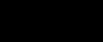
\includegraphics[width=0.7\columnwidth]{ultrametric_tree.pdf}
	\end{center}
	\caption[Ultrametric and non-ultrametric tree]{Ultrametric and non-ultrametric tree. The vertical components of the edges represent the distances. In the left tree, they induce an ultrametric on the set of its leaves, whereas they do not in the tree on the right side. This can, e.g., be seen by the violation of condition \textit{(iv*)} in Definition \ref{def:metric} for the leaves $x,y,z$: $d_2(x,y) > \max(d_2(x,z),d_2(z,y))$.}
	\label{fig:ultrametric_tree}
\end{figure}

In contrast, the distance function $d$ on the set of leaves $L(T)$ is not an ultrametric on the set of leaves in general. This is especially the case for evolutionary distances in the presence of asymmetric divergence as it will be discussed later. However, the distance function $d$ satisfies a weaker property by construction: A metric $d$ on set $X$ is \emph{additive} if a (not necessarily rooted) weighted tree $(T,\ell)$ exists such that $L(T)=X$ and $d=d_T$ where $d_T$ is the distance function of $(T,\ell)$ as defined by Equation~\ref{eq:distance_function}. A metric on a set $X$ can be tested for additivity with the four-point-condition: For any \emph{quartet}, i.e., a set of four nodes $x,y,u,v  \in X$, it must hold that out of the three distance sums
\begin{enumerate}[label=(\roman*), itemsep=0.2cm, topsep=0.2cm, parsep=0cm]
	\item $d(x,y)+d(u,v)$,
	\item $d(x,u)+d(y,v)$,
	\item $d(x,v)+d(y,u)$
\end{enumerate}
two sums are equal and not smaller than the third \citep[cf.][]{simoespereira1969,buneman1974}. 
The concept of quartets will be essential throughout this work:

\begin{definition}[Quartet Relation {\citep[cf.][]{stadler2020}}]
	\label{def:quartet_relation}
	Consider an unrooted tree $\unrooted{T}$ with leaf set $L(\unrooted{T})$. For any four distinct leaves $x,y,u,v\in L(\unrooted{T})$ denote by $\unrooted{T}[x,y,u,v]$ the unrooted tree obtained by suppressing all vertices of degree $2$ in the union of the paths in $\unrooted{T}$ that connect $x,y,u,v$. The \emph{quartet relation} for $\unrooted{T}$ is
	\begin{enumerate}[label=(\roman*), itemsep=0.2cm, topsep=0.2cm, parsep=0cm]
		\item $\unrooted{T}[x,y,u,v]=(xy|uv)$,
		\item $\unrooted{T}[x,y,u,v]=(xu|yv)$ or
		\item $\unrooted{T}[x,y,u,v]=(xv|yu)$
	\end{enumerate}
	if there is an edge $e\in E(\unrooted{T})$ such that the respective pairs (that are separated by the vertical bar) are in different connected components of $\unrooted{T}$ after the removal of $e$. If there is no such edge write $\unrooted{T}[x,y,u,v]=\times$.
\end{definition}

The four-point-condition is directly related to this notion of quartets: For an additive metric $d$, the smallest of the three distance sums induced by four distinct points $x,y,u$ and $v$ determines their topology in a corresponding tree $\unrooted{T}$ that explains $d$. The reason for this is that the edge separating two pairs in $\unrooted{T}[x,y,u,v]$ only contributes to the two larger sums. The case in which all three sums are equal corresponds to the absence of such a separating edge in $\unrooted{T}$ (and hence also in $\unrooted{T}[x,y,u,v]$) and is referred to as \emph{star tree} or \emph{star topology}. The possible cases are visualized in Figure~\ref{fig:possible_quartets_unrooted}.

\vspace{5mm}
\begin{figure}[ht]
	\begin{center}     
		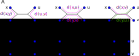
\includegraphics[width=0.9\columnwidth]{possible_quartets_unrooted.pdf}
	\end{center}
	\captionsetup{singlelinecheck=off}
	\caption[The four possible (unrooted) quartets]
	{The four possible (unrooted) quartets. For case (A), the six distances that form the three distance sums are indicated. In formal, the cases are:
		\begin{enumerate}[label=(\Alph*), itemsep=0.1cm, topsep=0.1cm, parsep=0cm]
			\item $\unrooted{T}[x,y,u,v]=(xy|uv)$ \newline $\iff d(x,y)+d(u,v) < d(x,u)+d(y,v) = d(x,v)+d(y,u)$
			\item $\unrooted{T}[x,y,u,v]=(xu|yv)$ \newline $\iff d(x,u)+d(y,v) < d(x,y)+d(u,v) = d(x,v)+d(y,u)$
			\item $\unrooted{T}[x,y,u,v]=(xv|yu)$ \newline $\iff d(x,v)+d(y,u) < d(x,y)+d(u,v) = d(x,u)+d(y,v)$
			\item $\unrooted{T}[x,y,u,v]=\times$ \newline $\iff d(x,y)+d(u,v) = d(x,u)+d(y,v) = d(x,v)+d(y,u)$
		\end{enumerate}
	}
	\label{fig:possible_quartets_unrooted}
\end{figure}

Given a rooted or unrooted tree $T$ and a unique numbering of the leaves $L(T)$, the distance function on the leaves can be represented by a symmetric square matrix which will be denoted by $\mathbf{D}$ in the following, where $\mathbf{D}(x,y)$ is the entry in the row and column corresponding to $x$ and $y$, respectively.



\subsection{Homology and Best Matches}
\label{sec:homology_and_bm}

As already outlined, the type of relationship between pairs of genes is of interest for the inference of gene functions. In particular, orthologous genes are considered to perform similar functions. Mathematically, both orthology and paralogy are binary relations on the set of (extant) genes in a gene tree $T$. They are defined w.r.t.\ the event type of the last common ancestor of two genes $x$ and $y$:

\begin{definition}[Orthology and Paralogy {\citep{fitch2000}}]
	\label{def:orthology}
	Let $(T,\mu,t)$ be an event-labeled, rooted gene tree with reconciliation map $\mu$.
	Two distinct leaves $x,y \in L(T)$ are \emph{orthologs w.r.t.\ $\mu$} if $t(\lca_T(x,y))=\SPEC$, and \emph{paralogs} if $t(\lca_T(x,y))=\DUPL$.
\end{definition}

Of course, the true reconciliation map and event-labeling are not known for real-life data. Therefore, methods exist that aim to explicitly reconstruct the gene tree and the reconciliation map, but also others that attempt to directly infer orthology based on gene similarity. In both cases, a well-founded mathematical investigation of the orthology and paralogy relation is helpful.

Firstly, Defintion~\ref{def:orthology} unambiguously defines two distinct members of a gene family as either orthologs or paralogs in the absence of horizontal gene transfer. Otherwise, there may be pairs of genes $x,y \in L(T)$ having a horizontal gene transfer as last common ancestor, and, thus, $t(\lca_T(x,y))=\HGT$.
Clearly, $x$ and $y$ are neither orthologs nor paralogs given the definition above. Therefore, \emph{xenology} was introduced as a third variant of homology. There are several definitions of xenologs. \citet{fitch2000} calls two genes xenologs if there is at least one HGT event on the unique path in $T$ connecting them. Thus, it is not necessary that their last common ancestor was an HGT event. As a consequence, two genes can be both xenologs and ortho-/paralogs. They are commonly termed as \emph{xeno-orthologs} and \emph{xeno-paralogs} in this case.
An alternative definition by \citet{hellmuth2016} avoids this ambiguity by calling two $x,y \in L(T)$ \emph{(lca-)xenologs} if and only if $t(\lca_T(x,y))=\HGT$. Analogously, \emph{(lca-)orthologs} and \emph{(lca-)paralogs} are defined. If not declared otherwise, all three terms will refer to this definition in the following.

Both orthology and paralogy are irreflexive and symmetric binary relations, since $t(\lca_T(x,x))=t(x)=\LEAF$ for any $x\in L(T)$ and $t(\lca_T(x,y)) = t(\lca_T(y,x))$ for any two genes $x,y\in L(T)$. Hence, they can be represented by undirected graphs. However, they are not transitive, as the example in Figure \ref{fig:ortho_para_example} shows (consider, e.g., the three genes $a_1,b_1,c_1$ in the orthology graph $\Theta$).
\begin{definition}[Orthology Graph {\citep[Def. 5 mod.]{geiss2020c}}]
	Let $T$ be a gene tree with event labeling $t$. Let $\Theta$ be the undirected graph on $L(T)$ with $xy \in E(\Theta)$ if and only if $\lca_T(x,y)=\SPEC$. Then $\Theta$ is called an \emph{orthology graph} that is explained by the orthology relation of $(T,t)$.
\end{definition}
Similarly, the paralogy graph $\overline{\Theta}$ is defined. In the absence of HGT events, it is simply the complement of $\Theta$.

\vspace{5mm}
\begin{figure}[H]
	\begin{center}     
		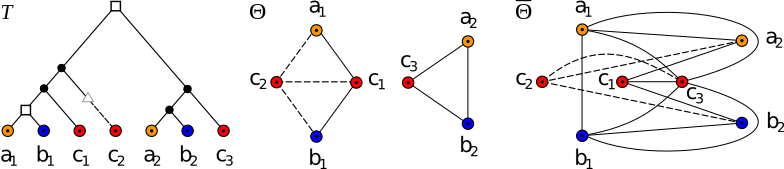
\includegraphics[width=\columnwidth]{ortho_para_example.pdf}
	\end{center}
	\caption[Example orthology graph $\Theta$ and paralogy graph $\overline{\Theta}$]{Corresponding orthology graph $\Theta$ and paralogy graph $\overline{\Theta}$ for the example gene tree in Figure \ref{fig:embedded_tree} restricted to the set of species $\{A,B,C\}$ (see tree $T$ on the left). Xeno-orthologous and \mbox{-paralogous} relations, respectively, are indicated by dashed lines.}
	\label{fig:ortho_para_example}
\end{figure}

Neither the orthology nor the paralogy relation can be observed directly. Therefore, heuristics have been developed that make use of the fact that orthologs are often the most closely related genes in two species. This approach has been used widely in phylogenetic reconstruction methods and requires some definition of the relationship between genes. To this end, different terms and variants have been introduced: Symmetric best matches \citep[e.g. used by][]{tatusov1997}, bidirectional best hits (BBH) \citep[e.g.][]{overbeek1999,lafond2018}, reciprocal best hits (RBH) \citep[e.g.][]{bork1998}, reciprocal best alignment heuristic (RBAH) \citep[e.g.][]{lechner2011} and some others.

To understand the aim of this work, it is necessary to strictly distinguish between \emph{best hits} and \emph{best matches}:

\begin{definition}[(Reciprocal) Best hit]
	\label{def:best_hit}
	Consider a gene tree $T$ with leaf set $L(T)$, a surjective map $\sigma\colon L(T)\to L(S)$ (where $L(S)$ is the corresponding set of species) and a distance function $d:L(T)\times L(T)\to \mathbb{R}_0^+$.  Then $y\in L(T)$ is a \emph{best hit} of $x\in L(T)$ if and only if $d(x,y)\le d(x,y')$ holds for all leaves $y'$ from species $\sigma(y')=\sigma(y)$.\newline
	If $x$ is also a best hit of $y$, $x$ and $y$ are called \emph{reciprocal best hits}.
\end{definition}

Thus, \emph{best hits} are defined in the context of the smallest evolutionary distance. On the other hand, \emph{best matches} refer to the closest relatives of a gene w.r.t.\ the point in time when they were separated:

\begin{definition}[(Reciprocal) Best match {\citep{geiss2019a}}]
	\label{def:best_match}
	Consider a gene tree~$T$ with leaf set $L(T)$ and a surjective map $\sigma\colon L(T)\to L(S)$ (where $L(S)$ is the corresponding set of species).  Then $y\in L(T)$ is a \emph{best match} of $x\in L(T)$, in symbols $x\rightarrow y$, if and only if $\lca(x,y)\preceq \lca(x,y')$ holds for all leaves $y'$ from species $\sigma(y')=\sigma(y)$.\newline
	If $x$ is also a best match of $y$ in color $\sigma(x)$, i.e., $y\rightarrow x$, $x$ and $y$ are called \emph{reciprocal best matches}.
\end{definition}

A comprehensive mathematical theory on best matches was developed only recently by \citet{geiss2019a}. Therein, the authors point out that best hits and best matches are the same if the mutation rate of the gene family is constant, i.e., the \emph{Molecular Clock} holds.

The best match relation can be represented by a directed, vertex-colored graph on the set of leaves of a gene tree $T$ as follows:

\begin{definition}[cBMG and cRBMG {\citep{geiss2019a}}]
	\label{def:cBMG}
	Given a gene tree $T$ and a map $\sigma:L(T)\to L(S)$, the \emph{colored Best Match Graph (cBMG)} $\protect\G(T,\sigma)$ has vertex set $L(T)$ and arcs $(x,y)\in E(\protect\G)$ if $x\ne y$ and $x\rightarrow y$. Each vertex $x\in L(T)$ obtains the color $\sigma(x)$.  \newline The rooted tree $T$ \emph{explains} the vertex-colored graph $(\protect\G,\sigma)$ if $(\protect\G,\sigma)$ is isomorphic (in the usual sense, with preservation of colors) to the cBMG $\protect\G(T,\sigma)$.\newline
	The vertex-colored undirected graph $G(T,\sigma)$ that has vertex set $L(T)$ and edges $xy\in E(G)$ if $x\ne y$ and $x\rightarrow y$ as well as $y\rightarrow x$ is called the \emph{colored Reciprocal Best Match Graph (cRBMG).}
\end{definition}

\citet{geiss2019a} present two polynomial-time algorithms to decide whether a given digraph $(\G,\sigma)$ is a valid colored Best Match Graph and to determine the unique least resolved tree, i.e., the corresponding tree which explains $(\G,\sigma)$ and is minimal in the sense that no edge can be contracted such that the tree still explains $(\G,\sigma)$. The algorithm for computing the least resolved tree that will be relevant later in this contribution makes use of informative triples:

\begin{definition}[Informative triples {\citep[Def.~8]{geiss2019a}}]
	\label{def:inftriples}
	Let $(\protect\G,\sigma)$ be a two-colored digraph. We say that a triple $ab|c$ is \emph{informative} (for $(\protect\G,\sigma)$) if the three distinct vertices $a,b,c\in L$ induce a colored subgraph $\protect\G[a,b,c]$ isomorphic (in the usual sense, with preservation of colors) to the graph $X_1$, $X_2$, $X_3$ or $X_4$ shown in Figure~\ref{fig:triples}. The set of informative triples is denoted by $\mathscr{R}(\protect\G,\sigma)$.
\end{definition}

\vspace{5mm}
\begin{figure}[ht]
	\begin{center}     
		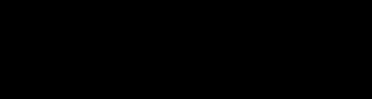
\includegraphics[width=0.85\columnwidth]{Triples.pdf}
	\end{center}
	\caption[Three-vertex induced subgraphs giving an informative triple]{Each of the three-vertex induced subgraphs $X_1$, $X_2$, $X_3$ and $X_4$ gives a triple $ab|c$. If vertex $c$ in the drawing has two colors, then the color $\sigma(c)$ does not matter \citep{geiss2019a}.}
	\label{fig:triples}
\end{figure}

This definition can easily be extended for n-colored graphs. \citet{geiss2019a} shows that the well-known polynomial-time algorithm \texttt{BUILD} \citep{aho1981} can be used to compute the least resolved tree directly from the full set of informative triples $\mathscr{R}(\protect\G,\sigma)$ of an n-colored Best Match Graph. Moreover, a colored digraph $(\G,\sigma)$ is a valid cBMG if and only if $(\G,\sigma) = \G(\textrm{Aho}(\mathscr{R}(\G,\sigma)),\sigma)$ where $\textrm{Aho}(\mathscr{R})$ denotes the tree $T$ that results from applying \texttt{BUILD} to a set of triples $\mathscr{R}$ \citep[][cf.~Theorems 6 and 9]{geiss2019a}. In other words, the Best Match Graph of the resulting tree has to be equal to the original digraph. Therefore, the explicit construction of a least resolved tree can be used to decide whether a given digraph is a cBMG.
%A more detailed description of Aho's \texttt{BUILD} algorithm and of the modification applied here will be given in the appropriate section (Section~\ref{sec:lrt_construction}).

\vspace{5mm}
In a subsequent publication, the properties of \emph{colored Reciprocal Best Match Graphs (cRBMG)} have been studied in detail \citep{geiss2020b}. Two genes $x$ and $y$ are reciprocal best matches if and only if both $x$ is a best match of $y$ and $y$ is a best match of $x$. As mentioned above, the cRBMG (possibly with some corrections based on the corresponding cBMG) is a good heuristic for the true orthology relation.
In fact, given a tree $T$ with reconciliation map $\mu$ and a corresponding event-labeling $t_\mu$, the orthology graph $\Theta(T,t_\mu)$ is a subgraph of the Reciprocal Best Match Graph $G(T,\sigma)$ \citep[Theorem~2]{geiss2020c} in the absence of horizontal gene transfer. Thus, the edges of $G$ cannot contain false positives w.r.t.\ the orthology relation.

Figure~\ref{fig:best_match_example} shows the cBMG $\G$, the cRBMG $G$ and the true orthology relation $\Theta$ that correspond to the previous example tree. The orthology graph is a subgraph of the cRBMG with exception of the xeno-orthologous relations. The simulations by \citet{geiss2020c} show that reciprocal best matches are a useful heuristic for orthology also if HGT occurs (at moderate rates).

\vspace{5mm}
\begin{figure}[ht]
	\begin{center}     
		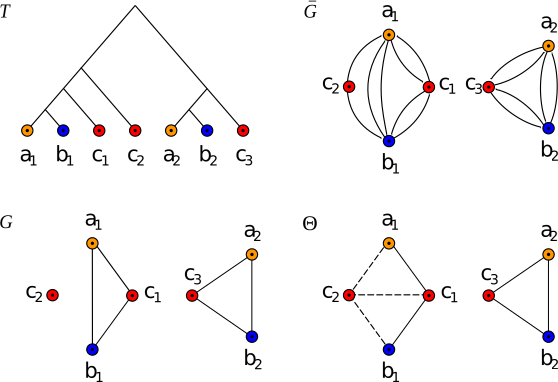
\includegraphics[width=0.9\columnwidth]{best_match_example.pdf}
	\end{center}
	\caption[Gene tree with corresponding cBMG and cRBMG]{Gene tree with corresponding colored Best Match Graph $(\G,\sigma)$ and Reciprocal Best Match Graph $(G,\sigma)$. The tree is a subtree of the gene tree in Figure~\ref{fig:embedded_tree} restricted to the set of species $\{A,B,C\}$. The true orthology graph $\Theta$ is again depicted for comparison.}
	\label{fig:best_match_example}
\end{figure}

However, especially in case of multiple losses, the true orthology relation is often hard to infer. The example includes the well-known problematic case of differential gene loss after a dupiclation event followed by speciation. The last common ancestor of genes $a_1$ and $b_1$ is a duplication (see Figure \ref{fig:embedded_tree}). The two loss events cause a false-positive edge when considering $G$ as the estimated orthology relation.
%It will be discussed later how the Best Match Graph can help resolve this issue in some cases (see Section~\ref{sec:role_best_matches}).

\bibliographystyle{plainnatnourl}
\bibliography{references}


\section*{Notation}
\addcontentsline{toc}{chapter}{Notation}

\vspace{5mm}
{\renewcommand{\baselinestretch}{1.12}\footnotesize
	\begin{minipage}[t]{0.47\textwidth}
		\textbf{Graphs}
		
		\vspace{2mm}
		\noindent
		$G=(V,E)$ -- undirected graph\\
		$V$ -- set of vertices\\
		$E$ -- set of edges\\
		$\G$ -- directed graph\\
		$x,y$ -- vertices\\
		$e,f$ -- edges\\
		$xy$ -- undirected edge between x and y\\
		$(x,y)$ -- directed edge between x and y\\
		$P$ -- path\\
		$\degree(x)$ -- degree of vertex $x$\\
		$\mathcal{C}$ -- set of connected components\\
		
		\noindent
		\textbf{(Phylogenetic) Trees}
		
		\vspace{2mm}
		\noindent
		$T=(V,E)$ -- rooted (gene) tree\\
		$T_{\textrm{obs}}$ -- observable gene tree\\
		$\unrooted{T}$ -- unrooted (gene) tree\\
		$S$ -- species tree\\
		$0_T, 0_S$ -- planted root\\
		$\rho_T, \rho_S$ -- root (first branching event)\\
		$u,v,w$ -- vertices\\
		$l, x, y, z$ -- genes / leaves\\
		$r, s, s_1, s_2$ -- species\\
		$\parent(v)$ -- parent of $v$\\
		$\child(v)$ -- set of children of $v$\\
		$V^0(T)$ -- inner vertices\\
		$L(T)$ -- leaves\\	
		$L[s]$ -- leaves of color/species $s$\\
		$T(v)$ -- subtree rooted at $v$\\
		$\preceq_T$ -- ancestor relation\\
		$\lca_T(A)$ -- last common ancestor of set $A$\\
		$xy|z$ -- rooted triple\\
		$(xy|uv)$ -- quartet relation\\
		$\sigma(x)$ -- leaf coloring map\\
		$\mu(v)$ -- reconciliation map\\
		$\tau(v)$ -- dating function\\
		$d_{\tau}(x,y)$ -- divergence time\\
		$\ell(e)$ -- length of edge $e$\\
		$d(x,y)$ -- (evolutionary) distance\\
		
		\noindent
		\textbf{Event labeling}
		
		\vspace{2mm}
		\noindent
		$t(v)$ -- event labeling map\\
		$\ROOT$ -- (planted) root\\
		$\LEAF$ -- leaf\\
		$\SPEC$ -- speciation\\
		$\DUPL$ -- duplication\\
	\end{minipage}
	\hfill
	\begin{minipage}[t]{0.47\textwidth}
		$\HGT$ -- horizontal gene transfer (HGT)\\
		$*$ -- loss\\
		
		\noindent
		\textbf{Orthology and Best Matches}
		
		\vspace{2mm}
		\noindent
		$\Theta$ -- (true) orthology graph\\
		$\unrooted{\Theta}$ -- (true) paralogy graph\\
		$\G$ -- colored Best Match Graph (cBMG)\\
		$G$ -- colored Reciprocal Best Match Graph (cRBMG)\\
		$x \rightarrow y$ -- best match relation\\
		$\left< a_1bca_2\right>$ -- induced $P_4$\\
		
		\noindent
		\textbf{Inference methods}
		
		\vspace{2mm}
		\noindent
		$\mathbf{D}$ -- distance matrix\\
		$\epsilon$ -- relative tolerance threshold\\
		$\eta$ -- discarding threshold for outgroup species\\
		$\mathscr{R}$ -- triple set\\
		$\mathscr{L}$ -- leaf set\\
		$\mathscr{H}$ -- auxiliary graph (\texttt{BUILD})\\
		$L_e$ -- leaf set (extant genes)\\
		$L_0$ -- leaf set (losses)\\
		$Z_v$ -- set of outgroups for vertex $v\in V(S)$\\
		
		\noindent
		\textbf{Simulation}
		
		\vspace{2mm}
		\noindent
		$d, l, h$ -- event rates\\
		$g\in G(\tau)$ -- extant gene at time $\tau$\\
		$q\in Q$ -- event type\\
		$\xi=(g,q)$ -- `reaction' in Gillespie algorithm\\
		$r_{\xi}(\tau)$ -- rate of reaction $\xi$\\
		$R(\tau)$ -- total rate\\
		$\Delta\tau$ -- waiting time\\
		$\mathcal{P}$ -- priority queue\\
		$K_A$ -- non-synonymous substitution rate\\
		$K_S$ -- synonymous substitution rate\\
		$\omega$ -- measure for selection pressure\\
		$R,R'$ -- asymmetry measures\\
		$\varrho$ -- evolution rate\\
		$k, \theta$ -- shape and scale (Gamma distribution)\\
		$\mathfrak{L}_e$ -- list of assigned rates to edge $e$\\
		$w_C, w_N, w_S$ -- weights for duplication types\\
		$\sigma$ -- standard deviation (normal distribution)\\
		$\alpha$ -- contribution of the disturbance matrix in a convex combination\\
		$\mathbf{D'}$ -- disturbed distance matrix\\
		$\mathfrak{S}$ -- standard simulated data set\\
		
	\end{minipage}
	
}

\end{document}
